\documentclass[12pt,a4paper]{scrartcl} 
\usepackage[utf8]{inputenc}
\usepackage[english,russian]{babel}
\usepackage{indentfirst}
\usepackage{misccorr}
\usepackage{graphicx}
\usepackage{amsmath}
\usepackage{titlesec}
\usepackage{tocbibind}
\usepackage{indentfirst} 
\setlength{\parindent}{1.25cm} 
\usepackage{setspace}

\titleformat{\section}
{\normalfont\Large\bfseries\centering} 
{\thesection.}                         
{0.5em}                                 
{}                                    

\titleformat{\subsection}
{\normalfont\large\bfseries}          
{\thesubsection}                      
{0.5em}                                 
{}                                  

\begin{document}
	\begin{titlepage}
		\begin{center}
			\large
			МИНИСТЕРСТВО НАУКИ И ВЫСШЕГО ОБРАЗОВАНИЯ РОССИЙСКОЙ ФЕДЕРАЦИИ
			
			Федеральное государственное бюджетное образовательное учреждение высшего образования
			
			\textbf{АДЫГЕЙСКИЙ ГОСУДАРСТВЕННЫЙ УНИВЕРСИТЕТ}
			\vspace{0.25cm}
			
			Инженерно-физический факультет
			
			Кафедра автоматизированных систем обработки информации и управления
			\vfill
			
			\vfill
			
			\textsc{Отчет по практике}\\[5mm]
			
			{\LARGE Программаная реализация численного метода Решение системы линейных алгебраических уравнений методом Крамера }
			\bigskip
			
			1 курс, группа ИВТ АСОИУ
		\end{center}
		\vfill
		
		\newlength{\ML}
		\settowidth{\ML}{«\underline{\hspace{0.7cm}}» \underline{\hspace{2cm}}}
		\hfill\begin{minipage}{0.5\textwidth}
			Выполнил:\\
			\underline{\hspace{\ML}} Д.\,Е.~Вакун\\
			«\underline{\hspace{0.7cm}}» \underline{\hspace{2cm}} 2025 г.
		\end{minipage}%
		\bigskip
		
		\settowidth{\ML}{«\underline{\hspace{0.7cm}}» \underline{\hspace{2cm}}}
		\hfill\begin{minipage}{0.5\textwidth}
			Выполнил:\\
			\underline{\hspace{\ML}} Я.\,Е.~Торотько\\
			«\underline{\hspace{0.7cm}}» \underline{\hspace{2cm}} 2025 г.
		\end{minipage}%
		\bigskip
		
		\settowidth{\ML}{«\underline{\hspace{0.7cm}}» \underline{\hspace{2cm}}}
		\hfill\begin{minipage}{0.5\textwidth}
			Выполнил:\\
			\underline{\hspace{\ML}} А.\,Е.~Удодов\\
			«\underline{\hspace{0.7cm}}» \underline{\hspace{2cm}} 2025 г.
		\end{minipage}%
		\bigskip
		
		\hfill\begin{minipage}{0.5\textwidth}
			Руководитель:\\
			\underline{\hspace{\ML}} С.\,В.~Теплоухов\\
			«\underline{\hspace{0.7cm}}» \underline{\hspace{2cm}} 2025 г.
		\end{minipage}%
		\vfill
		
		\begin{center}
			Майкоп, 2025 г.
		\end{center}
	\end{titlepage}
	
	

	\newpage 
	\tableofcontents 
	
	
	\newpage
	
	\section{Введение}

	Решение систем линейных алгебраических уравнений (СЛАУ) является одной из фундаментальных задач вычислительной математики и находит широкое применение в различных областях науки и техники, таких как физика, экономика, инженерные расчеты и многие другие. Существует множество методов решения СЛАУ, одним из классических является метод Крамера.
	
	\textbf{Целью данной работы} являлась разработка программного средства на языке C++ для решения систем линейных алгебраических уравнений методом Крамера для систем с числом неизвестных не более трех.
	
	Для достижения поставленной цели были решены \textbf{следующие задачи}:
	\begin{enumerate}
		\item Изучены теоретические основы метода Крамера, условия его применимости и алгоритм вычисления решения.
		\item Разработан алгоритм программы, включающий ввод исходных данных (матрицы коэффициентов и вектора свободных членов), вычисление необходимых определителей и нахождение вектора решения.
		\item Реализована программа на языке программирования C++, обеспечивающая пользовательский интерфейс для ввода данных и вывода результатов, а также контроль корректности вводимых значений.
		\item Проведено тестирование разработанной программы на примерах СЛАУ с известными решениями.
	\end{enumerate}
	
	В качестве инструмента для реализации был выбран язык программирования C++ благодаря его производительности и возможностям работы со структурами данных, необходимыми для представления матриц.
	
	\vspace{1ex} 
	
	В основе программной реализации лежит \textbf{метод Крамера}. Рассмотрим систему $n$ линейных алгебраических уравнений с $n$ неизвестными $x_1, x_2, \dots, x_n$:
	\[
	\left\{ 
	\begin{array}{@{}l@{}} 
		a_{11}x_1 + a_{12}x_2 + \dots + a_{1n}x_n = b_1 \\
		a_{21}x_1 + a_{22}x_2 + \dots + a_{2n}x_n = b_2 \\
		\multicolumn{1}{@{}c@{}}{\text{\Large$. \mspace{10mu} . \mspace{10mu} . \mspace{10mu} . \mspace{10mu} . \mspace{10mu} . \mspace{10mu} . \mspace{10mu} . \mspace{10mu} . \mspace{10mu} .$}} \\ 
		a_{n1}x_1 + a_{n2}x_2 + \dots + a_{nn}x_n = b_n
	\end{array}
	\right. 
	\]
	где $a_{ij}$ --- коэффициенты при неизвестных, а $b_i$ --- свободные члены ($i, j = 1, \dots, n$).
	
	Согласно методу Крамера, если главный определитель матрицы системы $\Delta \neq 0$, то система имеет единственное решение. Это решение для каждого неизвестного $x_i$ находится по формуле:
	\begin{equation}\label{eq:kramer} 
		x_i = \frac{1}{\Delta} \begin{vmatrix} 
			a_{11}   & \dots & a_{1,i-1}   & b_1    & a_{1,i+1}   & \dots & a_{1n}   \\
			a_{21}   & \dots & a_{2,i-1}   & b_2    & a_{2,i+1}   & \dots & a_{2n}   \\
			\dots    & \dots & \dots      & \dots  & \dots      & \dots  & \dots    \\ 
			a_{n-1,1} & \dots & a_{n-1,i-1} & b_{n-1} & a_{n-1,i+1} & \dots & a_{n-1,n} \\
			a_{n1}   & \dots & a_{n,i-1}   & b_n    & a_{n,i+1}   & \dots & a_{nn}   
		\end{vmatrix}
	\end{equation}
	где $\Delta$ --- главный определитель основной матрицы коэффициентов системы, а $\Delta_i$ (числитель дроби в формуле \eqref{eq:kramer_xi_in_intro}, если не выносить $\frac{1}{\Delta}$) представляет собой определитель матрицы, полученной из матрицы коэффициентов заменой $i$-го столбца столбцом свободных членов.
	
	Метод Крамера применим, если главный определитель системы $\Delta \neq 0$. Если $\Delta = 0$, система либо не имеет решений, либо имеет бесконечно много решений.
	

	\newpage
	
	\section{Ход работы}
	
	\subsection{Код приложения}
	\begin{verbatim}
		#include <iostream>
		#include <vector>
		#include <cmath>
		#include <limits>
		#include <iomanip>
		
		using namespace std;
		
		using Matrix = vector<vector<double>>;
		using Vector = vector<double>;
		
		
		void printMatrix(const Matrix& mat) // Функция для вывода матрицы на консоль.
		{
			if (mat.empty()) {
				cout << "Матрица пуста для вывода.\n";
				return;
			}
			for (const auto& row : mat) 
			{
				for (double val : row) 
				{
					cout << fixed << setprecision(2) << setw(8) << val << " ";
				}
				cout << endl;
			}
		}
		
		Matrix getMinor(const Matrix& mat, int skip_row, int skip_col) // Функция для 
		получения минора матрицы.
		{
			int n = mat.size();
			if (n <= 1) 
			{
				return Matrix();
			}
			Matrix minor(n - 1, vector<double>(n - 1));
			int r = 0;
			for (int i = 0; i < n; ++i) 
			{
				if (i == skip_row) continue;
				int c = 0;
				for (int j = 0; j < n; ++j) 
				{
					if (j == skip_col) continue;
					minor[r][c] = mat[i][j];
					c++;
				}
				r++;
			}
			return minor;
		}
		
		double calculateDeterminant(const Matrix& mat)// Рекурсивная функция для 
		вычисления определителя матрицы.
		{
			int n = mat.size();
			
			if (n == 1) 
			{
				return mat[0][0];
			}
			
			if (n == 2) 
			{
				return mat[0][0] * mat[1][1] - mat[0][1] * mat[1][0];
			}
			
			double determinant = 0;
			for (int k = 0; k < n; ++k) 
			{
				Matrix minor = getMinor(mat, 0, k);
				determinant += pow(-1, k) * mat[0][k] * calculateDeterminant(minor);
			}
			return determinant;
		}
		
		Matrix createMatrixForKramer(const Matrix& A, const Vector& b, 
		int columnIndexToReplace)// Функция для создания вспомогательной матрицы для 
		метода Крамера. 
		{
			int n = A.size();
			if (n == 0 || A[0].size() != n || b.size() != n) 
			{
				cerr << "Ошибка: Некорректные размеры матрицы A или вектора b для 
				createMatrixForKramer.\n";
				return Matrix();
			}
			
			Matrix Ak = A;
			for (int i = 0; i < n; ++i) 
			{
				Ak[i][columnIndexToReplace] = b[i];
			}
			return Ak;
		}
		
		int main() 
		{
			setlocale(LC_ALL, "Russian");
			cout << "Программа для решения СЛАУ методом Крамера.\n";
			
			int n;
			while (true) 
			{
				cout << "Введите порядок системы (количество неизвестных n не должно превышать 
				3): ";
				if (!(cin >> n)) 
				{
					cout << "Ошибка ввода. Пожалуйста, введите целое число.\n";
					cin.clear();
					cin.ignore(numeric_limits<streamsize>::max(), '\n');
				}
				else if (n <= 0 || n >= 4) 
				{
					cout << "Порядок системы должен быть 1, 2 или 3.\n";
				}
				else 
				{
					break;
				}
			}
			
			Matrix A(n, Vector(n));
			Vector b(n);
			Vector x(n);
			
			cout << "Введите элементы матрицы коэффициентов A (" << n << "x" << n << "):\n";
			for (int i = 0; i < n; ++i) 
			{
				for (int j = 0; j < n; ++j) 
				{
					while (true) 
					{
						cout << "A[" << i + 1 << "][" << j + 1 << "]: ";
						if (!(cin >> A[i][j])) 
						{
							cout << "Ошибка ввода. Пожалуйста, введите число.\n";
							cin.clear();
							cin.ignore(numeric_limits<streamsize>::max(), '\n');
						}
						else 
						{
							break;
						}
					}
				}
			}
			
			cout << "Введите элементы столбца свободных членов b (" << n << "x1):\n";
			for (int i = 0; i < n; ++i) 
			{
				while (true) 
				{
					cout << "b[" << i + 1 << "]: ";
					if (!(cin >> b[i])) 
					{
						cout << "Ошибка ввода. Пожалуйста, введите число.\n";
						cin.clear();
						cin.ignore(numeric_limits<streamsize>::max(), '\n');
					}
					else 
					{
						break;
					}
				}
			}
			
			cout << "\nВведенная матрица A:\n";
			printMatrix(A);
			cout << "\nВведенный столбец свободных членов b:\n";
			for (int i = 0; i < n; ++i) 
			{
				cout << "b[" << i + 1 << "] = " << fixed << setprecision(2) << b[i] << endl;
			}
			
			double detA = calculateDeterminant(A);
			cout << "\nГлавный определитель системы det(A) = " << fixed << 
			setprecision(4) << detA << endl;
			
			const double epsilon = 1e-9;
			if (abs(detA) < epsilon) 
			{
				bool all_det_i_zero = true;
				for (int j = 0; j < n; ++j) 
				{
					Matrix Aj = createMatrixForKramer(A, b, j);
					if (abs(calculateDeterminant(Aj)) > epsilon) 
					{
						all_det_i_zero = false;
						break;
					}
				}
				if (all_det_i_zero) 
				{
					cout << "Система имеет бесконечно много решений (det(A)=0 и все det(Aj)=0)." 
					<< endl;
				}
				else 
				{
					cout << "Система не имеет решений (det(A)=0 и хотя бы один det(Aj)!=0)."
					 << endl;
				}
			}
			else 
			{
				cout << "\nРешения системы (x_i = det(A_i) / det(A)):\n";
				for (int j = 0; j < n; ++j) 
				{ 
					Matrix Aj = createMatrixForKramer(A, b, j);
					
					double detAj = calculateDeterminant(Aj);
					x[j] = detAj / detA;
					cout << "x[" << j + 1 << "] = " << fixed << setprecision(4) << detAj << " / " 
					<< detA << " = " << x[j] << endl;
				}
				
				cout << "\nВектор решений x:\n";
				for (int i = 0; i < n; ++i) 
				{
					cout << "x[" << i + 1 << "] = " << fixed << setprecision(4) << x[i] << endl;
				}
			}
			
			return 0;
		}
	\end{verbatim}
	
	\subsection{Тестирование программы}
	
	Для проверки корректности работы разработанной программы была решена тестовая система линейных алгебраических уравнений.
	
	\vspace{1.5ex}
	
	\noindent\textbf{Тестовый пример} 
	\vspace{1ex}
	
	Рассмотрим следующую систему из трех линейных алгебраических уравнений с тремя неизвестными, которая была использована для тестирования:
	\[
	\begin{cases} 
		2x_1 + 3x_2 + 5x_3 = 43 \\
		32x_1 + 88x_2 + 12x_3 = 23 \\
		6x_1 + 3x_2 + x_3 = 76
	\end{cases}
	\]
	
	Для данной системы в программу были введены следующие значения:
	\begin{itemize}
		\item Матрица коэффициентов $A$:
		\[ A = \begin{pmatrix} 
			2 & 3 & 5 \\
			32 & 88 & 12 \\
			6 & 3 & 1 
		\end{pmatrix} \]
		\item Вектор свободных членов $b$:
		\[ b = \begin{pmatrix} 
			43 \\ 23 \\ 76 
		\end{pmatrix} \]
	\end{itemize}
	
	\vspace{1ex} 
	
	После запуска программы и ввода указанных данных были получены следующие результаты для вектора решений $x$:
	\begin{verbatim}
		Вектор решений x:
		x[1] = 14.5620
		x[2] = -5.8946
		x[3] = 6.3120
	\end{verbatim}
	
	Для проверки корректности полученных программой значений, они были сравнены с ожидаемыми результатами, рассчитанными с помощью онлайн калькулятора "Решение систем линейных уравнений методом Крамера". Ожидаемые значения для данной системы:
	\begin{itemize}
		\item $x_1 \approx 14.5620$
		\item $x_2 \approx -5.8946$
		\item $x_3 \approx 6.3120$
	\end{itemize}
	
	Сравнение показывает, что результаты, выданные программой, хорошо согласуются с ожидаемыми значениями.
	
	\textbf{Вывод по тестовому примеру:} Разработанная программа корректно решает заданную систему линейных алгебраических уравнений методом Крамера, что подтверждается совпадением полученных результатов с ожидаемыми.
	
	\newpage
	
	\section{Демонстрация работы программы} 
	
	Ниже на рисунке 1 представлен пример консольного вывода программы при решении системы линейных алгебраических уравнений. На скриншоте отображен процесс ввода данных пользователем и итоговый результат, выданный программой.
	
	\begin{figure}[h!]
		\centering
		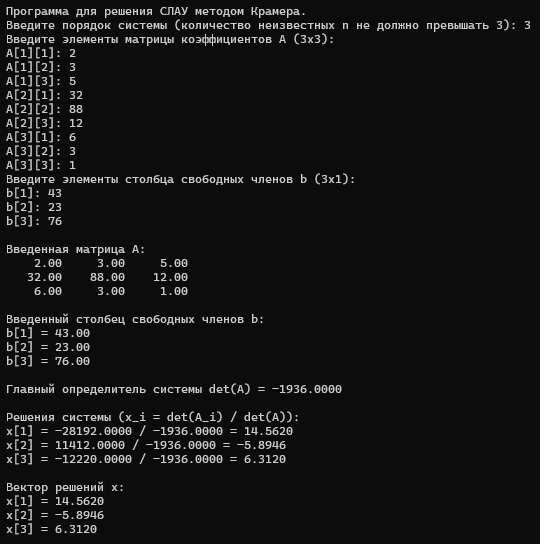
\includegraphics[width=0.7\textwidth]{Демонстрация работы программы.png}
		\caption{Пример вывода консоли при работе программы}
	\end{figure}
	
	\newpage
	
	\begin{thebibliography}{6}
		
		\bibitem{ilin_poznyak_linal_kramer}
		Ильин В.А., Позняк Э.Г. Линейная алгебра: Учебник. --- 6-е изд., стер. --- М.: ФИЗМАТЛИТ, 2007. --- 280 с. 

		\bibitem{beklemishev_linal_detailed}
		Беклемишев Д.В. Курс аналитической геометрии и линейной алгебры: Учебник для вузов. --- 12-е изд., испр. --- М.: ФИЗМАТЛИТ, 2008. --- 312 с. 
		
		\bibitem{kostrikin_algebra_tom1}
		Кострикин А.И. Введение в алгебру. В 3-х томах. Том 1. Основы алгебры: Учебник для вузов. --- 3-е изд., испр. и доп. --- М.: ФИЗМАТЛИТ, 2004. --- 272 с.
		
		\bibitem{voevodin_linal}
		Воеводин В.В. Линейная алгебра: Учебное пособие. --- М.: Наука, 1980. --- 400 с. 

		
		\bibitem{gelphand_lectures_linal}
		Гельфанд И.М. Лекции по линейной алгебре: Учебник. --- 5-е изд., испр. --- М.: Добросвет, МЦНМО, 2009. --- 280 с.
		
		\bibitem{proskuryakov_linal}
		Проскуряков И.В. Сборник задач по линейной алгебре: Учебное пособие. --- 13-е изд., стер. --- СПб.: Лань, 2010. --- 480 с.
		
	\end{thebibliography}
	
\end{document}
